Las visualizaciones interactivas web se implementan combinando un conjunto variado de tecnologías: HTML para el contenido de la página, CSS para la apariencia, JavaScript para la interacción, SVG para los gráficos vectoriales, entre otros. Estas tecnologías funcionan de manera integrada sobre la representación compartida de la página llamada Modelo de Objetos de Documento (DOM) \cite{Bos11}.

Actualmente existen toolkits que aprovechan estas tecnologías para la generación de visualizaciones de datos. El toolkit apropiado para cada caso debe seleccionarse tomando en consideración los requerimientos del proyecto, como por ejemplo el tipo de visualización, la tecnologías a usar, tiempo de desarrollo disponible y hasta la compatibilidad con navegadores, entre otros. Murray \cite{Mur13} clasifica los toolkits disponibles de la siguiente manera:

\begin{itemize}
  \item Librerías de gráficos prediseñados
  \item Librerías para gráficos específicos (grafos, geomapping, etc.)
  \item Librerías para el diseño de visualizaciones 2D
  \item LIbrerías para el diseño de visualizaciones 3D
\end{itemize}

En este capítulo se presentan las más recientes especificaciones de las tecnologías fundamentales para la visualización, que incluyen HTML, CSS, DOM, scripting (JavaScript) y gráficos (PNG, SVG, Canvas, WebCGM). Por último se presentan aquellos toolkits que permiten el dibujar gráficos vectoriales sin limitarse a plantillas prediseñadas (D3.js, Processing.js, Raphael.js, Paper.js).

\section{Fundamentos tecnológicos}

\subsection{HTML}

HTML es el lenguaje de marcado para definir la estructura de las páginas web \cite{HnC13}. Está compuesto por elementos que definen el tipo de contenido que va a ser desplegado por el navegador y son a su vez estructuras semánticas que describen la función de cada parte del documento sin ambigüedad \cite{Wp14}. El estándar HTML es mantenido por W3C (World Wide Web Consortium) \cite{MozHTML}.

En un documento HTML un elemento se denota mediante un par de etiquetas, una inicial y otra final, como se muestra en el fragmento de código \ref{sniphtml}. Un elemento puede contener otros elementos o texto. La información adicional asociada a un elemento se agrega mediante atributos colocados en la etiqueta inicial. En el Algoritmo \ref{sniphtml} se muestra como se puede usar el atributo 'class' para proporcionar información semántica sobre el elemento.

\lstinputlisting[language=HTML,label=sniphtml,caption={[Fragmento de código HTML] Fragmento de código HTML \cite{HnC13}}]{snippets/snippet.html}

HTML5 es la quinta revisión del estándar HTML. Esta especificación intenta resolver las fallas que las anteriores tenían en el área de las aplicaciones web, ofreciendo un lenguaje de marcado y un conjunto de scripting APIs enfocados en la semántica \cite{Html5}. En cuanto al lenguaje de marcado, se introduce una conjunto de elementos y atributos nuevos entre los cuales están \cite{Diff13}:

\begin{itemize}
  \item Los semánticos, que son aquellos enfocados en mejorar la estructura del documento, como por ejemplo section, nav y header;
  \item Los multimedia, enfocados en eliminar las dependencias de plugins propietarios. Entre ellos están vídeo, audio y canvas;
  \item Los de formulario, que agregan un conjunto de valores (tel, email, url, color, etc.) al atributo 'type' del elemento 'input'. Esto mejora la experiencia de usuario ya que su entrada es validada antes  de ser enviada al servidor, reduciendo así el tiempo de respuesta.
\end{itemize}

Entre los APIs ofrecidos están aquellos para el control de video y audio, validación de formularios y el canvas 2D, entre otros. El Canvas API es una tecnología de scripting que permite la creación y alteración de imágenes rasterizadas (bitmaps). Debido a que no tiene DOM, puede ejecutarse con bastante rapidez. Es soportado de manera nativa en la mayoría de los navegadores modernos en incluso en dispositivos móviles \cite{Gra13}.

\subsection{CSS}

Según la W3C CSS es un "mecanismo sencillo para agregar estilo (tipografía, color y espaciado) a documentos web" \cite{HnC13}. Las hojas de estilo CSS ofrecen control sobre el formato y la disposición de un documento basado en XML. CSS trabaja sobre un sistema de reglas las cuales seleccionan un elemento que requiere de formato y luego establece valores a las diferentes propiedades del elemento \cite{Wp14}.

Una de las grandes ventajas de CSS es que permite la separación de estructura (HTML) y presentación (CSS), y con ello se simplifica el mantenimiento de una página, se promueve la reutilización de hojas de estilo y la se facilita la adaptación de páginas a diferentes entornos \cite{HnC13}.

La sintaxis de CSS posee dos bloques básicos de construcción: la propiedad, que es un identificador, y el valor, el cual describe como esta propiedad debe ser manejada por el motor del navegador (ver Algoritmo \ref{snipcss}). La funcionalidad principal de CSS es de establecer un valor específico a una propiedad. Un par propiedad-valor se denomina declaración. El par es separado por dos puntos. Las declaraciones son agrupadas en bloques delimitados por llaves, mejor llamados bloques de declaración. Cada bloque de declaración está precedido por un selector que es una condición que selecciona algunos elementos de la página. El par selector-bloque de declaración es lo que se conoce como regla \cite{MozCSS}.

\lstinputlisting[label=snipcss,caption={[Fragmento de código CSS] Fragmento de código CSS \cite{Wp14}}]{snippets/snippet.css}

Las hojas de estilo pueden declararse dentro de un elemento HTML, dentro de la sección 'head' de un documento HTML o en un archivo CSS externo. Para determinar qué estilo va a ser usado cuando hay más de un estilo declarado para un mismo elemento HTML, se sigue lo que se conoce como orden de escascadamiento. En él los estilos prevalecen según el siguiente orden de prioridad ascendente \cite{CssHT}:

\begin{itemize}
  \item Estilo predefinido del navegador
  \item Hoja de estilo externa
  \item Estilos en la sección 'head' del documento HTML
  \item Estilos dentro del elemento HTML
\end{itemize}

CCS3 es la última revisión del lenguaje CSS y tiene como objetivo extender la especificación CSS2.1. Ofrece un conjunto de novedades como lo son los bordes redondeados, las sombras, las transiciones y nuevas plantillas de disposición. Permite adaptar la presentación de la página web a los distintos tipos de dispositivos \cite{MozCSS3}.

\subsection{DOM}

El modelo de objetos de documento (DOM) es una interfaz independiente de la plataforma y el lenguaje que permite a los programas y scripts el acceso dinámico y la actualización del contenido, estructura y estilo de documentos \cite{Rob98}. El DOM se crea al momento de cargar una página y es construido como un objeto con estructura de árbol \cite{JsHD}, como se muestra \figlink{fig:fig18}{}. El DOM provee una representación del documento como una estructura de nodos que posee propiedades, métodos y manejadores de eventos. El DOM esencialmente conecta la página web a los scripts o lenguajes de programación \cite{MozDOM}.

\begin{figure}[htp]
  \centering
  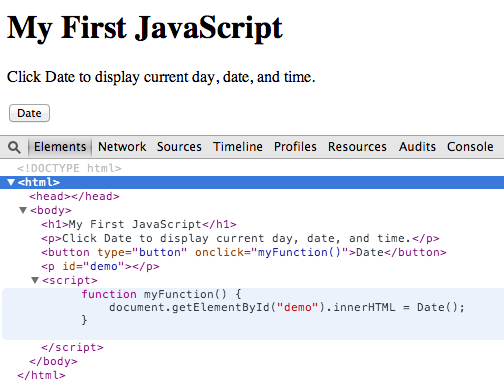
\includegraphics[width=0.85\textwidth]{fig18.png}
  \caption[Modelo de objetos de documento (DOM)]{El árbol DOM del algoritmo \ref{snipjs} obtenido con "Google Chrome Web Inspector"}
  \label{fig:fig18}
\end{figure}

\subsection{JavaScript}

Un script es un código de programa que no necesita de preprocesamiento (compilación) para su ejecución. En el contexto de un navegador web, el scripting se refiere por lo general a códigos de programa escritos en JavaScript que son ejecutados por el navegador cuando una página es descargada, o en respuesta a un evento provocado por el usuario \cite{Js13}.

JavaScript es un lenguaje interpretado, liviano, basado en prototipos y multiparadigma que soporta la programación orientada a objetos, imperativa y funcional \cite{MozJS}.

JavaScript hace las páginas web más dinámicas al permitir modificar, agregar y enviar contenido desde la página sin tener que cargarla nuevamente. Adicionalmente, permite crear puentes de comunicación entre el navegador y la plataforma en donde corre, haciendo posible la incorporación de información local del ambiente del usuario \cite{Js13}.

Haciendo uso del DOM, JavaScript puede crear HTML dinámico de la siguiente manera \cite{JsHD}:

\begin{itemize}
  \item Cambiando los elementos HTML
  \item Cambiando los atributos HTML
  \item Cambiando los estilos CSS
  \item Eliminando elementos y atributos HTML existentes
  \item Añadiendo nuevos elementos y atributos HTML
  \item Reaccionando a eventos HTML
  \item Creando nuevos eventos HTML
\end{itemize}

El Algoritmo \ref{snipjs} es un ejemplo de una página HTML que haciendo uso de JavaScript muestra la fecha y hora local luego de presionar un botón.

\lstinputlisting[language=HTML,label=snipjs,caption={[Fragmento de código JavaScript] Fragmento de código JavaScript \cite{JsTut}}]{snippets/snippetjs.html}

\subsection{SVG}

SVG es el lenguaje de marcado XML para describir gráficos de aplicación e imágenes de 2 dimensiones y un conjunto de interfaces de scripts gráficos \cite{Svg10}.Comprende aspectos como la geometría de las formas, el estilo del texto, las animaciones y presentaciones multimedia (video, audio, etc.). Es totalmente interactivo y posee un DOM que permite scripting. Soporta un amplio rango de transformaciones visuales como gradientes, opacidad, filtros, recortes y máscaras \cite{Gra13}.

Usando SVG se pueden crear gráficos de alta calidad, completamente escalables y reusables; desde gráficos simples hasta potenciar páginas webs, desde diagramas interactivos hasta visualizaciones de datos. SVG es soportado por todos los browser modernos y está disponible para una gran variedad de dispositivos móviles.

El Algoritmo \ref{snipsvg} es un ejemplo del uso de SVG para dibujar un círculo con un gradiente que simula el efecto de profundidad
\lstinputlisting[language=XML,label=snipsvg,caption={[Fragmento de código SVG] Fragmento de código SVG \cite{Gra13}}]{snippets/snippet.svg}

\subsection{D3.js}

D3 es una librería de JavaScript que permite la inspección y manipulación directa del modelo de objetos del documento (DOM) \cite{D3JS}. Fue desarrollada por Mike Bostock bajo la licencia BSD y se encuentra disponible en Github \footnote{\url{https://github.com/mbostock/d3}}. Con D3, el diseñador de manera selectiva vincula los datos de entrada a elementos arbitrarios del documento y luego aplica transformaciones dinámicas al contenido generado \cite{Bos11}. Las transformaciones en D3 facilitan la implementación de visualizaciones dinámicas mediante control explícito de los elemento del modelo de objetos de dominio (DOM) y la evaluación inmediata de operadores sobre dichos elementos.

D3 no es un framework monolítico que busca proveer todas las funcionalidades posibles. De lo contrario, se enfoca en la manipulación eficiente de un documentos en base a datos. Esto evita las representaciones propietarias y permite extraordinaria flexibilidad, exponiendo las capacidades de los estándares web como CSS3, HTML5 y SVG \Fig{fig:fig19}{}. D3 es extremadamente rápido, soporta grandes conjuntos de datos y comportamiento dinámico para interacciones. El estilo funcional de D3 garantiza códigos reusable y una amplia colección de componentes y plugins \cite{D3JS}. D3 es soportado por Firefox, Chrome, Safari, Opera, IE9+, Android and iOS \cite{GitD3}.

\begin{figure}[htp]
  \centering
  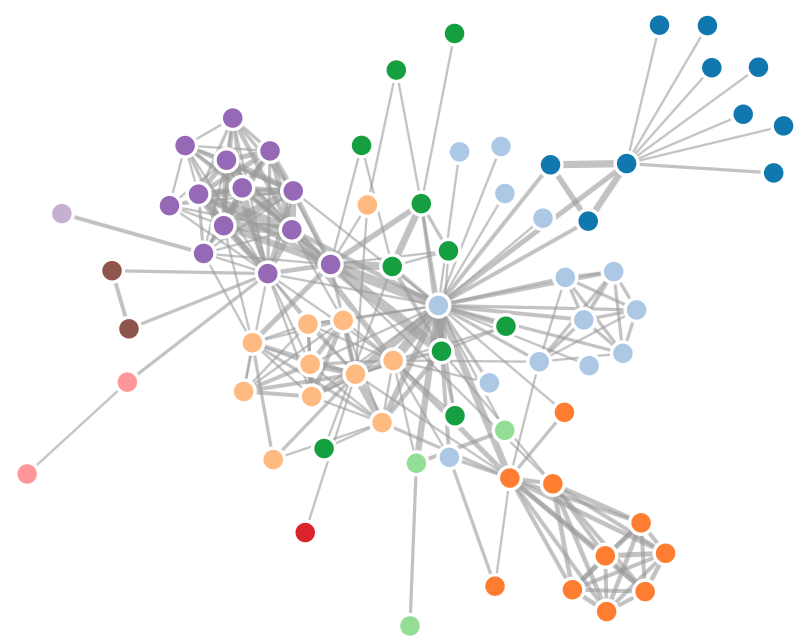
\includegraphics[width=0.7\textwidth]{fig19.png}
  \caption[Visualización de la aparición simultánea de personajes en Les Misérables usando D3.js]{Visualización de la aparición simultánea de personajes en Les Misérables mediante un grafo dirigido por fuerza \protect\footnotemark. Una simulación física de partículas y puentes cargados colocan a personajes relacionados en cercana proximidad, mientras que los personajes no relacionados están más separadas.}
  \label{fig:fig19}
\end{figure}

\footnotetext{Tomada de: \url{http://bl.ocks.org/mbostock/4062045}}

\subsection{Raphael.js}

Es una librería de JavaScript para trabajar de manera sencilla con gráficos vectoriales en la Web \cite{RaphJS}. Fue desarrollada por Dmitry Baranovski y se encuentra alojada en Github \footnote{\url{https://github.com/DmitryBaranovskiy/raphael}}. Permite hacer tareas como crear gráficos personalizados, cortar imágenes y rotar widgets. Básicamente provee un API para la manipulación de SVG y el soporte de SVG para Internet Explorer \cite{Bar09}. Cada objeto que se crea es también un objeto DOM que puede modificarse posteriormente o adjuntársele manejadores de eventos de JavaScript. Esto permite la creación de visualizaciones interactivas y animaciones \Fig{fig:fig20}{}. Raphael soporta Firefox 3.0+, Safari 3.0+, Chrome 5.0+, Opera 9.5+ e Internet Explorer 6.0+.

\begin{figure}[htp]
  \centering
  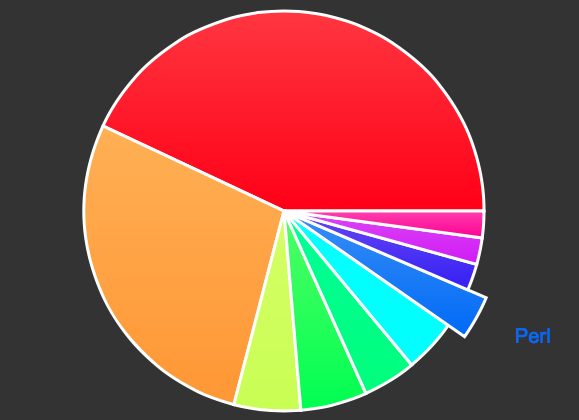
\includegraphics[width=0.6\textwidth]{fig20.png}
  \caption[Demo "Languages" de la libreria Raphael.js]{Demo "Languages" de la libreria Raphael.js \protect\footnotemark. Visualización de un gráfico de tortas sobre el uso de lenguajes de progamación.}
  \label{fig:fig20}
\end{figure}

\footnotetext{Tomada de: \url{http://raphaeljs.com/pie.html}}

\subsection{Processing.js}

Processing.js es la implementación web del popular lenguaje de programación Processing. Permite hacer visualizaciones de datos \Fig{fig:fig21}, arte digital, animaciones interactivas, gráficos educativos, juegos de video, entre otros, usando estándares web y sin necesidad de plugins \cite{ProcJS}. Para usarlo simplemente se escribe el código en lenguaje de Processing (o su versión en JavaScript), se incluye en la página web y se importa Processing.js \footnote{Disponible en: \url{https://github.com/processing-js/processing-js}} la cual se encarga de la implementación. La librería es compatible con cualquier navegador conforme con HTML5, incluyendo las versiones recientes de Firefox, Safari, Chrome, Opera e Internet Explorer.

Processing es un lenguaje de programación que consiste de un entorno de desarrollo, una colección de funciones y métodos, una sintaxis casi idéntica a Java y una comunidad en línea \cite{Fry07}. Un programa de Processing se llama un sketch, e implementa una programación escrita en Java que se siente más como el scripting, y que es más accesible a una audiencia más amplia que solo programadores, tales como artistas y diseñadores gráficos.

\begin{figure}[htp]
  \centering
  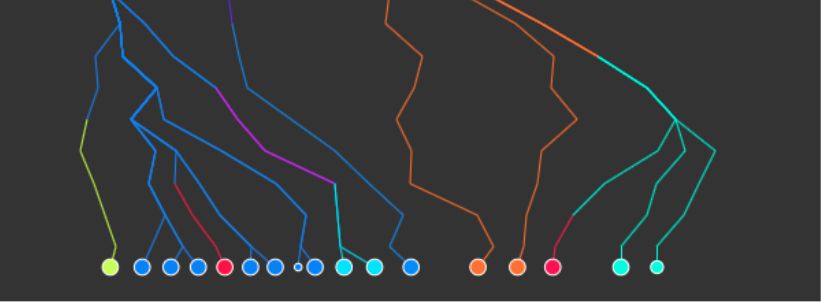
\includegraphics[width=0.75\textwidth]{fig21.png}
  \caption[Simulación de un árbol genealógico usando partículas cargadas usando Processing.js]{Simulación de un árbol genealógico usando partículas cargadas \protect\footnotemark. Los individuos nacen creando lineages linajes que se ramifican y desaparecen cuando los individuos mueren.}
  \label{fig:fig21}
\end{figure}

\subsection{Paper.js}

\footnotetext{Tomada de: \url{http://bedford.io/projects/coaltrace/}}

Es un framework de código abierto para gráficos vectoriales que se ejecuta encima de HTML5 Canvas \cite{PaperJS}. Paper.js fue desarrollada por Jürg Lehni y Jonathan Puckey y distribuida \footnote{\url{https://github.com/paperjs/paper.js}} bajo la licencia MIT. Provee una interfaz de programación consistente y limpia con funcionalidades poderosas para crear y trabajar con gráficos vectoriales y curvas de bezier. Permite construir trayectorias y manipular sus curvas y segmentos de una manera conveniente y con gran precisión. Apunta a navegadores modernos que tengan soporte de Canvas y de ECMAScript5.

\begin{figure}[htp]
  \centering
  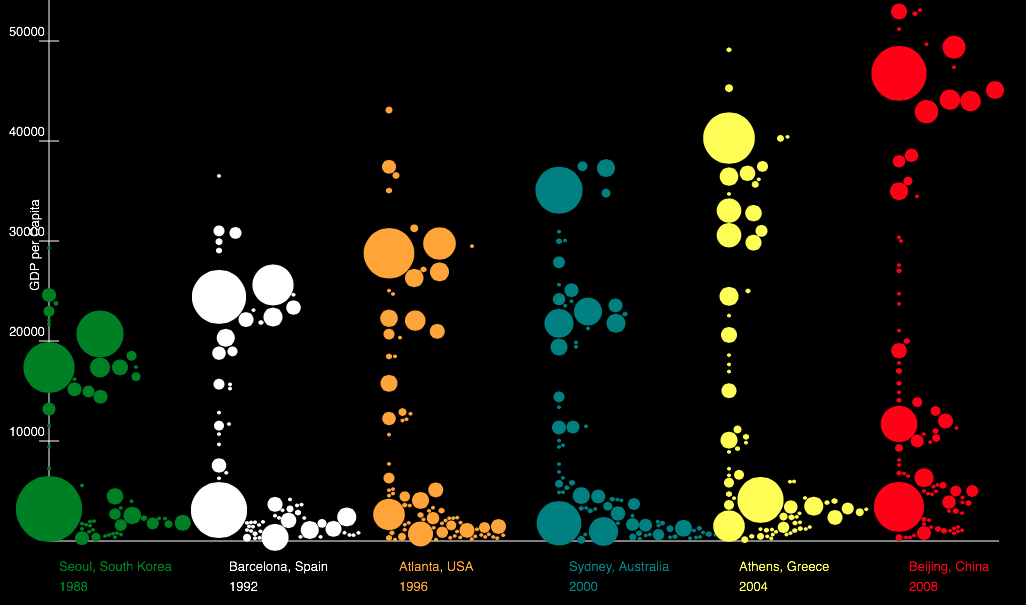
\includegraphics[width=0.75\textwidth]{fig22.png}
  \caption[Visualización de medallas en las Olimpiadas usando Paper.js]{Visualización de los últimos 6 juegos olímpicos de verano y total de medallas de cada país \protect\footnotemark}
  \label{fig:fig22}
\end{figure}

\footnotetext{Tomada de: \url{https://github.com/nandayadav/olympics_visualization}}
